\section{Slackline learning techniques}\label{3_3_learningTechniques}
Subsection \textit{\nameref{2_1_1_slacklineTraining}} showed that systematic help is not essentially necessary for learning slacklining. The user for the interactive learning system should therefore be able to learn it by herself without any further external help. To achieve this two learning concepts will be differentiated in subsection \textit{\nameref{3_3_1_learningConcepts}}. Further specific slackline exercises can be categorized like described in subsection \textit{\nameref{3_3_2_StagesExercises}}, which structures at the same time the learning flow of the user.

\subsection{Methods for slackline skill acquisition}\label{3_3_1_learningConcepts}
\subsubsection{Methodical routine}
A methodical routine can be integrated in almost every sport activity. For this a series of exercises is chosen. With further practise their difficulty is increasing. The chosen exercises are based on methodical principals that can be for example defined with easy to difficult, known to unknown, or simple to complex exercises~\cite{Fetz1996-ml}. Größing~\cite{Groessing1997-sp} describes it as follows. At the beginning of this methodical routine the trainee will execute warm up exercises. This can be useful to prepare her for the training. After that preliminary exercise will be provided, which are more specific regarding the actual exercises. With this she will learn the general motoric basics and train the movements needed to perform the activity. Further it ensures a smooth transition for the main exercises.

For slacklining skill acquisition Thomann~\cite{Thomann2013-aa} developed a methodical routine as well as an dynamical methodic. The methodical routine can be seen in figure \ref{fig:3_3_1_methodicalRoutine} and inherits various approaches with different elements to reach the goal of learning slacklining. Because there is variability in the integration of the elements, each tutor can build her one routine and choose different aspects. At first, like already explained, an introduction and preliminary exercises can be integrated, which follows by material and security. In here the lines dynamic, how to jump off and controlling of the line should be covered. Following the learning of the oscillation behaviour should be implemented with or without methodical help. The same can be distinguished in the next aspect, which involves the decision of balance training. With help the trainee can directly balance on the line with providing external support. Without any further help she can decide to first sit, step on the line, or independent balance. Continuing one has to decide if first the static or dynamical balance has to be trained. Following the trainee has the possibility to train more variable with exercises like walking forwards on the line, walking backwards, with eye closed, etc. Before going to train some tricks on the line, which is on the very end of the routine, the trainee has to learn first staying across the line with her feet. This is a necessary part of various tricks and has to be learned before.

\begin{figure}[htb]
	\centering
	\begin{minipage}[t]{1\linewidth}
		\centering
		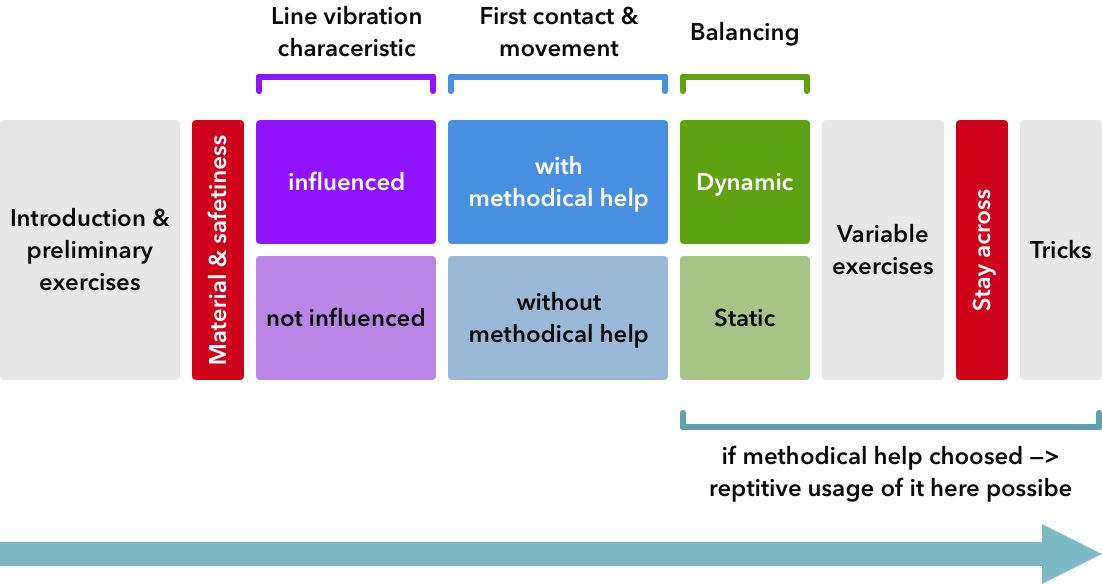
\includegraphics[width=1\linewidth]{Pictures/3_3_1_methodicalRoutine3}
		\caption{Methodical routine~\cite{Thomann2013-aa}}
		\label{fig:3_3_1_methodicalRoutine}
	\end{minipage}
\end{figure}

\subsubsection{Differential methodic}
The differential or dynamic methodic follows another approach. It is in coherence of an open learning situation~\cite{Thomann2013-aa}. This means it depends on several factors, which in slacklining would be line type, line length, tension, environment, etc. According to the interplay of these factors each trainee can construct her own training set. A dynamic methodic is a practical usage for this~\cite{Beck2008-dl, Schoellhorn1999-ip}. This inherits the model of stepping stones. In general it describes that many possibilities can lead to the same goal. Each potential way has therefore its own difficulty level. This results in a more dynamic way to reach that goal. In comparison to the methodical routine it results in bigger differences in stimulus, like compared in figure~\ref{fig:3_3_1_comparisonMethods}. 

\begin{figure}[htb]
	\centering
	\begin{minipage}[t]{1\linewidth}
		\centering
		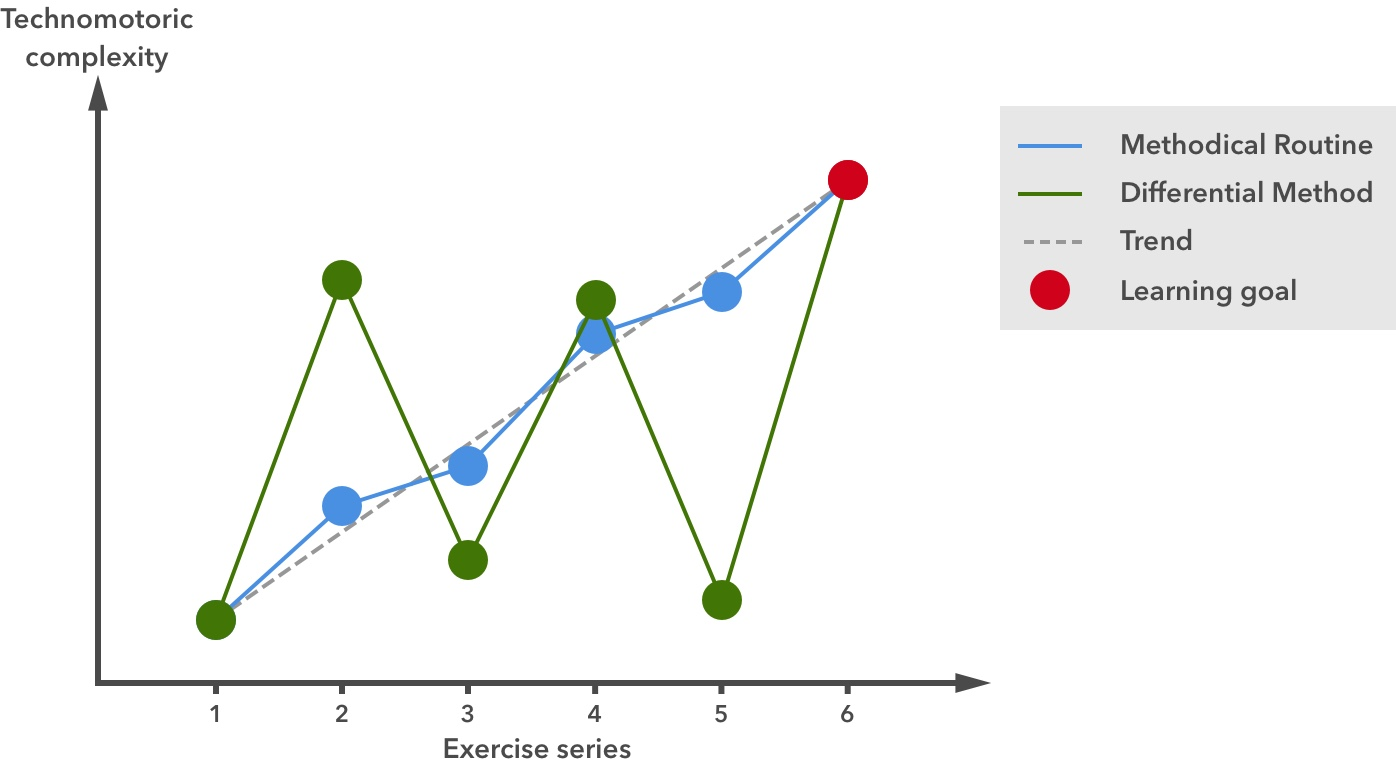
\includegraphics[width=1\linewidth]{Pictures/3_3_1_comparisonMethod2}
		\caption{Comparison methodical routine vs. differential method~\cite{Thomann2013-aa}}
		\label{fig:3_3_1_comparisonMethods}
	\end{minipage}
\end{figure}
At first the trainee can follow a methodical principle like seen in methodical routine. If she reaches a certain threshold of skill level more dynamic procedures can be involved in the actual learn process. Therefore the principle of differential learning can be used in which results in big stimulus differences and provide more variability in the movement execution.

The usage in slacklining can be integrated like described and visualized by Thomann~\cite{Thomann2013-aa} (Figure \ref{fig:3_3_1_dynamicMethod}). On the x-axis the complexity of the exercise is given, whereas on the y-axis various learning stages. The goal is described in the upper right corner. The goal is to choose an amount of various exercise of all stages. Each more complex exercise can either integrate methodical support or the trainee can return to the lower stage for movement training for the specific exercise. With this an individual way can be formed for each trainee. Modification and integration of more useful exercises are also allowed. Structured examples can be seen in figure~\ref{fig:3_3_1_dynamicMethod}. The black arrows visualize a way for people that are more coordinative, more venturesome, or have background knowledge. In contrasat the blue arrows visualize a path for people that are less coordinate, less venturesome, or have no background knowledge in slacklining.

\begin{figure}[htb]
	\centering
	\begin{minipage}[t]{1\linewidth}
		\centering
		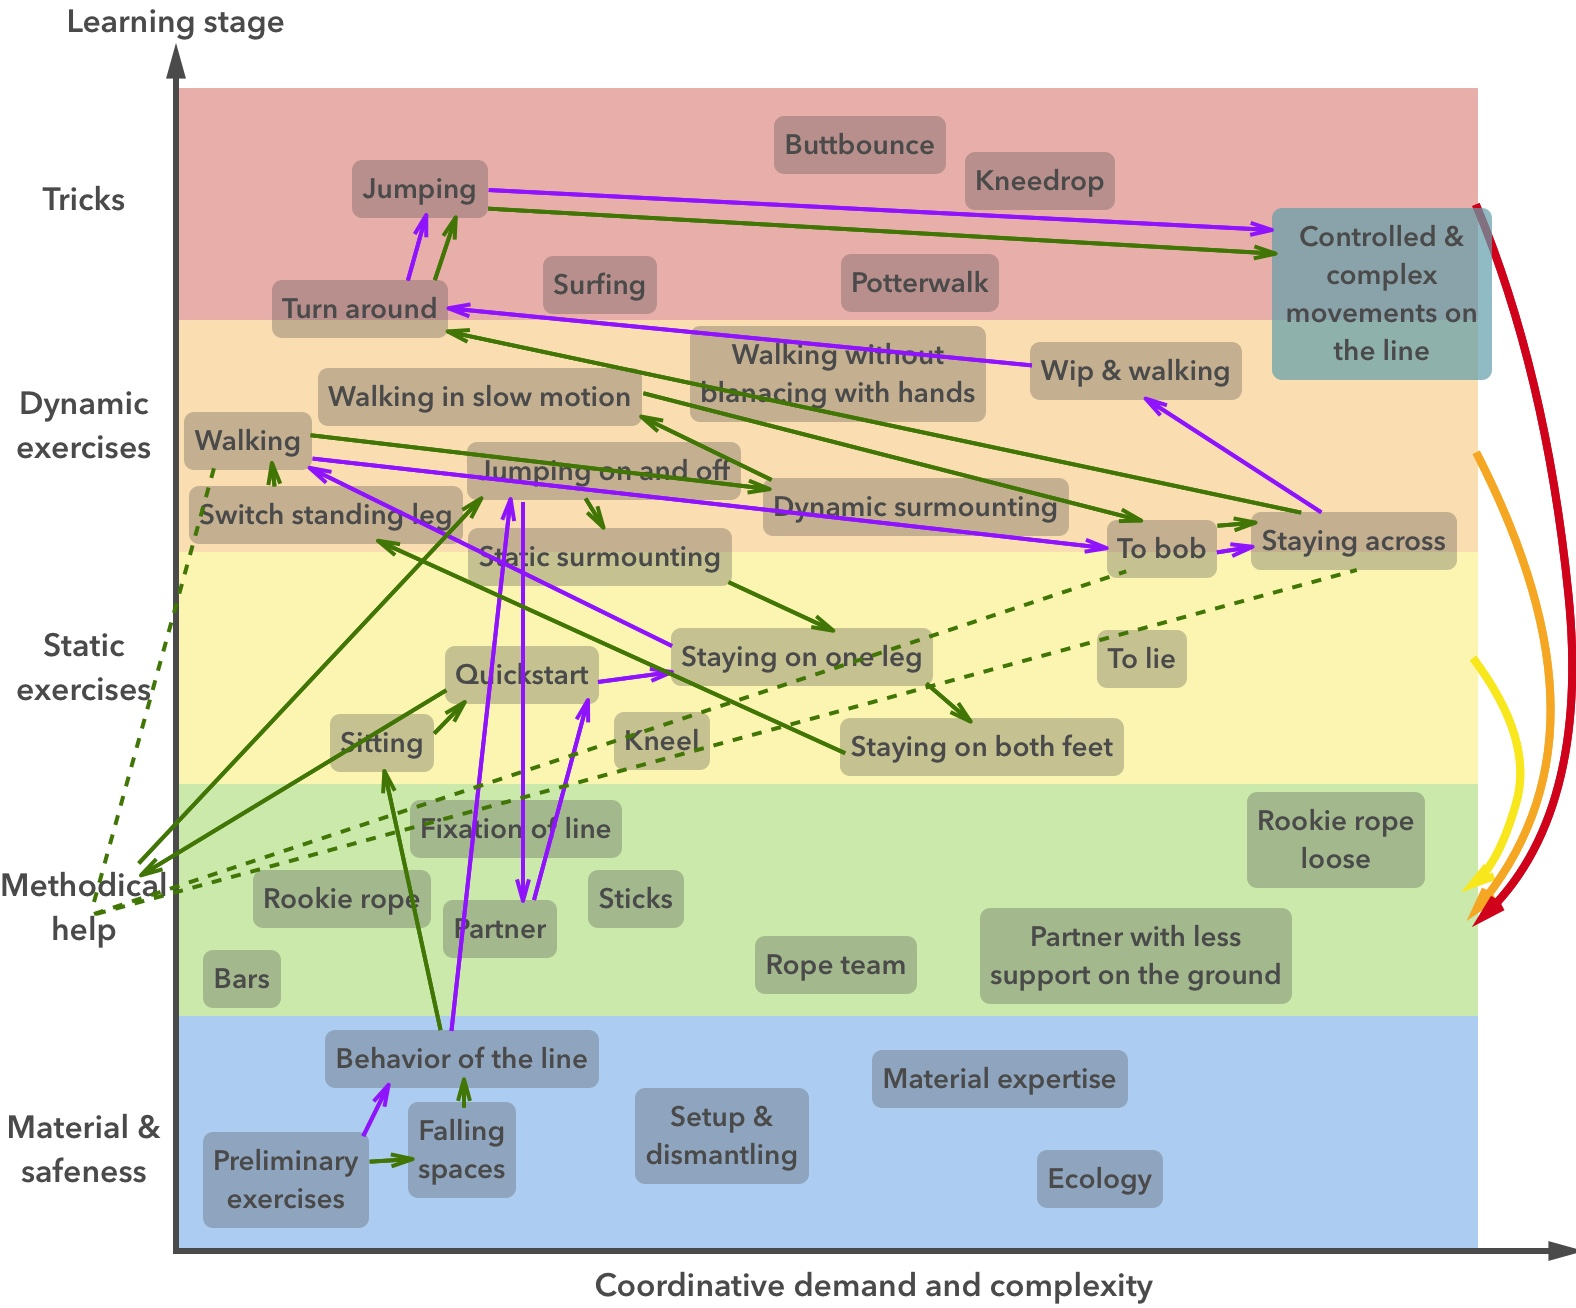
\includegraphics[width=1\linewidth]{Pictures/3_3_1_dynamicMethod3}
		\caption{Dynamic methodic in slacklining~\cite{Thomann2013-aa}}
		\label{fig:3_3_1_dynamicMethod}
	\end{minipage}
\end{figure}

For proper user training with the system the trainee should follow a clear workflow. As a first approach for a prototype the methodical routine is the better choice as a learning concept in an interactive learning system. It follows a clear linear workflow, in which stages and exercises can be designed as levels. The trainee can unlock further levels by successfully executing the prior exercise. Also he learns right from the beginning essential aspects of slacklining that are relevant and build up on each other. 
The next subsection \textit{\nameref{3_3_2_StagesExercises}} will therefore cover a clear workflow integration of exercises for a learning system.

\subsection{Stages and exercise of learning slacklining}\label{3_3_2_StagesExercises}
% Drei verschiedene Grundfertigkeiten: zunächst muss man auf einem Bein stehen können, dazu kommt die schmale Unterstützungsfläche, auf der man balancieren soll. Nicht zuletzt befindet man sich in einer gewissen Höhe und nicht mehr auf sicherem Boden.
Now that an overview about slacklining and its learning techniques are given several practical exercises have to be considered. Repetitive trials are one approach of learning to walk on the line. However this could result in dangerous situations and frustration of the slacker because of her missing skills. Therefore an exercise set has to be considered that teach and guide the slacker to reach her goal. The teaching goal should be that the slacker can balance with a controlled manner on the line and be able to walk a few steps on it. In general to be able achieve this one has to acquire three core skills~\cite{Kroiss2007-ab}. At first the slacker should be able to stay on one foot. This is essential because most of the time the slacker has a standing foot on the line and the other foot servers as balance component. Second the balancing on a narrow surface since the slackline exists of a limited width. Lastly managing the height is also important due to the fact that the slackline is mostly tensed around the knee height and above.

As a groundwork the elaborated exercises are based on Kroiß~\cite{Kroiss2007-ab}. He elicited slacklining learning exercises for beginners within a school class, which gives a good basic on the exercise integration. Furhter several other references~\cite{Balcom2005-wl, Donath2013-kk, Donath2016-gm, Granacher2010-ow, Keller2012-xh, Kleindl2011-bl, Pfusterschmied2013-yy, Thomann2013-aa} have been researched to elaborate exercises that fit the best in this system. Each exercise is therefore categorized in one of four tiers, which represent the fundamental basis of the exercises routine. In the following each tier is introduced, its goal clarified, and the learning aspects described.

\subsubsection{Tier I - Preliminary exercises}
The first tier severs as a preparation for the subsequent exercises. In here just exercises on the ground will be executed. This is to train and strengthen the slacker general physical balance. In general it is recommended to train barefoot or with socks to have a better feeling in the foot. The knees should be bent to have a better initial position for movement compensation. Keeping the head up and setting a focus point can help to calm the visual sense of balance. In almost all exercises of this tier the arms have to be stretched to the side, be over the shoulder and bent in about 135 degree. This is the biggest balance function overall because you have freedom in all directions and it can shift the body's center of gravity. Further all exercises should be executed slowly and controlled to master your body behaviour.

\subsubsection{Tier II - First contact with the line}
Mastering the general physical balancing leads the slacker to her first experience with the slackline. The goal is to get a feeling for the slackline and to be able to get up on the line and hold herself for a short amount of time. For this the slacker has to become familiar with the line, feel the imbalance, how the body wants to behave, and get a feeling for counterbalancing unpredictable movements. Therefore starting at the sweet spot, that's about 1/3 of the line, can help. It's an area with a comfortable vibration characteristic. The foot should be always in alignment with the slackline to have the biggest amount of surface of your foot covered with the line, which results in more contact. If the slacker has problems with holding her hands over the shoulder, she can turn the palms to the top and the hands will then raise automatically up. A relaxed but straight upper body can help to hold the right position.

\subsubsection{Tier III - Static exercises}
In here the exercises are getting more difficult. The slacker is now familiar with the line and able to stand for a short amount of time on it. This tier has the goal that the slacker should stay confidently on the line and it serves as preparation for walking on the line. All prior learned techniques have to be directly applied. The non standing leg now comes more into action. It serves as an addition balancing parameter to both of the arms. If the slacker has problems with going up on the line, she can keep the balancing leg vertically in line with the standing leg while up going and then move it to the side. The pressure is mostly around the ball of the foot.

\subsubsection{Tier IV - Dynamic exercises}
This is the last tier and it involves the dynamical part for the slackline. The slacker should now be able to stay confidently on the line with one foot and both feet. The goal is to learn how to make the first steps as a result for walking on the line. In general it is applying static exercises together. While staying on the line and when the slacker wants to make a step she can guide her balancing foot to the side of the line and shift it then forwards. Letting the knees together when making a step forward helps because the legs can support each other. Making small steps won't shift the body's center of gravity that much forward, which results in more control.
